\section{Implementation}
With the full algorithm of the back propagation a full Neural Network could be developed. You can do it by following the steps and code it in \textit{Python}, \textit{Haskell}, \textit{Matlab} \dots But as you develop your net you will notice that it is only valid for a certain network architecture, and it is pretty slow because of the languages. You can develop it on \textit{C++} or even in \textit{C} what will need a lot of effort for achieving more speed.

But as Neural Networks are not new and as they are well known and famous, there are many tools you can choose for creating your model. It will be much faster to implement it and the net will run also faster since the tools are optimized. One of the most famous tools is developed by \textit{Google}. They are the kings of de big data and they are using the data for machine learning so they have created \textit{TensorFlow} carefully to fullfill all their needs.

\subsection{Tensorflow}
TensorFlow is an open source software library for numerical computation using data flow graphs. It was developed initially for \textit{Google} machine learning purposes but it could be used in other domains. It was released for the first time in 2015 and now it is on version \textit{1.4.0}. This tool gives you a APIs of different levels of abstraction that allow you to work with complex numerical computation in an abstract, easy and elegant way ~\cite{amy}.

In TensorFlow \textbf{SIN ACABAR}

\subsection{MNIST Data Set}
Every time you start learning a new language you first start with \textit{Hello World}. In the machine learning this program is the \textit{MNIST} problem. The \textit{MNIST} data set is composed by 70.000 images of handwritten digits (See Figure ~\ref{fig:mnist}), and the whole data set has been studied several times as it has shown to fit very well with basic neural networks.

\begin{figure}
  \center
  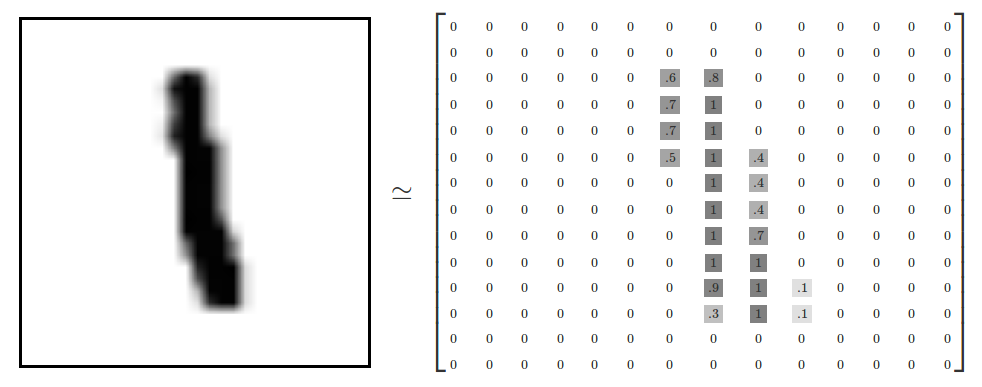
\includegraphics[scale=0.4]{images/MNIST-Matrix.png}
  \caption{The images are $28x28$ pixels where each of them describes how dark is that point of the image. This figure is $14x14$ for simplicity ~\cite{colah} }
  \label{fig:mnist}
\end{figure}

In order to be able to give the images to the input they are stored as flattened vector of $24\cdot24=784$ numbers. The output of the networ will be an array of dimension $10$ where each position is $0$ but one has the value $1$. The position of the value $1$ represents which number the network thinks the image is. For instance, if the input is the image of a $8$ the perfect output is $[0,0,0,0,0,0,0,0,1,0]$.

\subsection{Building the Model}
As we have seen from the data the input is of dimension $784$ while the output has $10$ outcoming values. We are going to have two hidden layers of 256 neurons each. We are going to define the parameters of the network so we also can define the learning constant $\alpha=0.01$, the number of epochs to $1000$ and the batch size (number of images the network train with in each epoch) to $100$.

\begin{lstlisting}[language=python]
#Network parameters
n_hidden1 = 256
n_hidden2 = 256
n_input = 784
n_output = 10
#Learning parameters
learning_constant = 0.01
number_epochs = 1000
batch_size = 100
\end{lstlisting}

We also have to specify how we are going to input the data and how we expect the ouput, for that we are goin gto define the placehoders, defining that the input is a two dimensions array of floats, one dimension is every input (784) and as we do not know the number of images we are going to give we write \textit{None} for the other dimension. In a similar way the output is defined.

\begin{lstlisting}[language=python]
X = tf.placeholder("float", [None, n_input])
Y = tf.placeholder("float", [None, n_output])
\end{lstlisting}

Each neuron has a bias and each pair of neurons of neighbours layers has a weight so we must define all of them:
\begin{lstlisting}[language=python]
#Biases first hidden layer
b1 = tf.Variable(tf.random_normal([n_hidden1]))
#Biases second hidden layer
b2 = tf.Variable(tf.random_normal([n_hidden2]))
#Biases output layer
b3 = tf.Variable(tf.random_normal([n_output]))

#Weights connecting input layer with first hidden layer
w1 = tf.Variable(tf.random_normal([n_input, n_hidden1]))
#Weights connecting first hidden layer with second hidden layer
w2 = tf.Variable(tf.random_normal([n_hidden1, n_hidden2]))
#Weights connecting second hidden layer with output layer
w3 = tf.Variable(tf.random_normal([n_hidden2, n_output]))
\end{lstlisting}

Done, we have defined $728\cdot256+256\cdot256+256\cdot10=254464$ weights in three lines, TensorFlow is powerful. To finish we just have to tell how the four layers are connected, and the the model will be ready to be trained. To achieve it we have to define what is the task for each neuron. If one vector of data $x$ is incoming to a neuron, it has to weight it ($w$) add the bias $u$ and apply the activation function $f(x\cdot W+u)$. Making the product of each input data with their weight is as simple as applying \textit{tf.matmul}, then add the bias with \textit{tf.add} and finally apply the activation function \textit{tf.nn.relu}.
\begin{lstlisting}[language=python]
#The incoming data given to the
#network is input_d
def multilayer_perceptron(input_d):
    #Task of neurons of first hidden layer
    layer_1 = tf.nn.relu(tf.add(tf.matmul(input_d, w1), b1))
    #Task of neurons of second hidden layer
    layer_2 = tf.nn.relu(tf.add(tf.matmul(layer_1, w2), b2))
    #Task of neurons of output layer
    out_layer = tf.add(tf.matmul(layer_2, w3),b3)
    return out_layer
\end{lstlisting}

The full neural network model can be stored in a single variable in such a simple way as (\textit{X} is the placeholder we have already defined as the input of the network):
\begin{lstlisting}[language=python]
# Create model
neural_network = multilayer_perceptron(X)
\end{lstlisting}
\subsection{Training the Model}
Is the moment of training the network. For that purpose we have to define what is the error and which method we are going to use to fix it. The error or the loss is calculated giving our model and the placeholder of the output. For fixing that loss we are going to apply the gradient descent optimizer and we have to define what we want to reduce and what is the learning constant.

\begin{lstlisting}[language=python]
#Define the loss or the error
loss_op = tf.reduce_mean(tf.nn.softmax_cross_entropy_with_logits(
                         logits=neural_network,labels=Y))
#Define how to fix it
optimizer = tf.train.GradientDescentOptimizer(learning_constant)
                      .minimize(loss_op)
\end{lstlisting}

Next step is iterate trought all the epochs. In each one the program should take one batch of images and their expected output, feed the network with it, and finally apply the optimizer we have already defined. The task of running the epochs could not be done in such a simple way as we have defined the model. The train should be performed inside a TensorFlow session after all the declares variables are initialized. The session allows not just declare the model but perform operations.

\begin{lstlisting}[language=python]
#Initializing the variables
init = tf.global_variables_initializer()
#Create a session
with tf.Session() as sess:
    sess.run(init)
    #Training epoch
    for epoch in range(number_epochs):
        #Get one batch of images
        batch_x, batch_y = mnist.train.next_batch(batch_size)
        #Run the optimizer feeding the network with the batch
        sess.run(optimizer, feed_dict={X: batch_x, Y: batch_y})
        #Display the epoch (just every 100)
        if epoch % 100 == 0:
            print("Epoch:", '%d' % (epoch))
\end{lstlisting}

\subsection{Evaluating the Model}
The network is already trained so it is the time of test how well we have designed it and how much it has learned. One part of the date set was reserved for testing. The outputs of the network are not as perfect as one vector with all $0$ but one $1$ pointing the solution. Actually it is more close to something like $[0.01,0.94,0.02,0.025,0.025,0.06,0.01,0.01,0.4,0.04]$ because the network is not absolutely sure about the answer so the output is something like "I am 94\% sure that this is a 1 but it could be a 8 in a 4\% and a bit percentage for the other options". To transform that answers the \textit{softmax} function should be applied. It takes the bigger number and transform it to a $1$ while change the other smallers numbers with $0$s. Now we define what is a correct answer with \textit{tf.equal}, one prediction is correct if it is equal to the expected output, easy. To finish we define the accuracy to print it and feed the network wiht the test subset.

\begin{lstlisting}[language=python]
# Test model
pred = tf.nn.softmax(neural_network)  # Apply softmax to logits
correct_prediction = tf.equal(tf.argmax(pred, 1), tf.argmax(Y, 1))
# Calculate accuracy
accuracy = tf.reduce_mean(tf.cast(correct_prediction, "float"))
print("Accuracy:", accuracy.eval({X: mnist.test.images, Y: mnist.test.labels}))
\end{lstlisting}

If we execute the code we get an accuracy close to 90\%. It might seem that is a great result, it answer correctly 9 out of 10 times. But in machine learning this result is pretty bad, it is normal because the network used is the most simple network but compared with other kind of models it is a bit shaming.
